\documentclass{beamer}
\usepackage[utf8]{inputenc}
  
\usetheme{Madrid}
\usecolortheme{default}
\usepackage{amsmath,amssymb,amsfonts,amsthm}
\usepackage{txfonts}
\usepackage{tkz-euclide}
\usepackage{listings}
\usepackage{adjustbox}
\usepackage{array}
\usepackage{tabularx}
\usepackage{gvv}
\usepackage{lmodern}
\usepackage{circuitikz}
\usepackage{tikz}
\usepackage{graphicx}
\usepackage[T1]{fontenc}
\UseRawInputEncoding

\setbeamertemplate{page number in head/foot}[totalframenumber]

\usepackage{tcolorbox}
\tcbuselibrary{minted,breakable,xparse,skins}



\definecolor{bg}{gray}{0.95}
\DeclareTCBListing{mintedbox}{O{}m!O{}}{%
  breakable=true,
  listing engine=minted,
  listing only,
  minted language=#2,
  minted style=default,
  minted options={%
    linenos,
    gobble=0,
    breaklines=true,
    breakafter=,,
    fontsize=\small,
    numbersep=8pt,
    #1},
  boxsep=0pt,
  left skip=0pt,
  right skip=0pt,
  left=25pt,
  right=0pt,
  top=3pt,
  bottom=3pt,
  arc=5pt,
  leftrule=0pt,
  rightrule=0pt,
  bottomrule=2pt,
  toprule=2pt,
  colback=bg,
  colframe=orange!70,
  enhanced,
  overlay={%
    \begin{tcbclipinterior}
    \fill[orange!20!white] (frame.south west) rectangle ([xshift=20pt]frame.north west);
    \end{tcbclipinterior}},
  #3,
}
\lstset{
    language=C,
    basicstyle=\ttfamily\small,
    keywordstyle=\color{blue},
    stringstyle=\color{orange},
    commentstyle=\color{green!60!black},
    numbers=left,
    numberstyle=\tiny\color{gray},
    breaklines=true,
    showstringspaces=false,
}



\title 
{MatGeo Assignment 4.4.3}

\author
{AI25BTECH11007}
\begin{document}

\frame{\titlepage}
\begin{frame}{Question}
Find the values of $\lambda$ for which the distance of the point (2, 1, $\lambda$) from the plane\\
3x + 5y + 4z = 11 is $2\sqrt{2}$ units.
\end{frame}

\begin{frame}{Solution}
\[
\text{Plane: } 3x+5y+4z=11 
\quad\Rightarrow\quad 
\vec{n}=\myvec{3\\5\\4}.
\]

Let point be 
\[
\vec{p}=\myvec{2\\1\\\lambda}.
\]

The distance of a point \(\vec p\) from plane \(\vec n^T\vec x=11\) is
\begin{equation}
d=\frac{|\vec n^T\vec p-11|}{\|\vec n\|}.
\end{equation}

Now,
\begin{equation}
\vec {n}^T\vec {p}
= \myvec{3 & 5 & 4}\myvec{2\\1\\\lambda} 
= 11+4\lambda,
\end{equation}
    
\end{frame}
\begin{frame}
and
\begin{equation}
\|\vec n\|
= 5\sqrt{2}.
\end{equation}

Hence,
\begin{equation}
d=\frac{|11+4\lambda-11|}{5\sqrt{2}} = 2\sqrt{2}.
\end{equation}

\begin{equation}
\therefore \quad \lambda=\pm 5.
\end{equation}
\end{frame}

\begin{frame}{Plot}
\begin{figure}
    \centering
    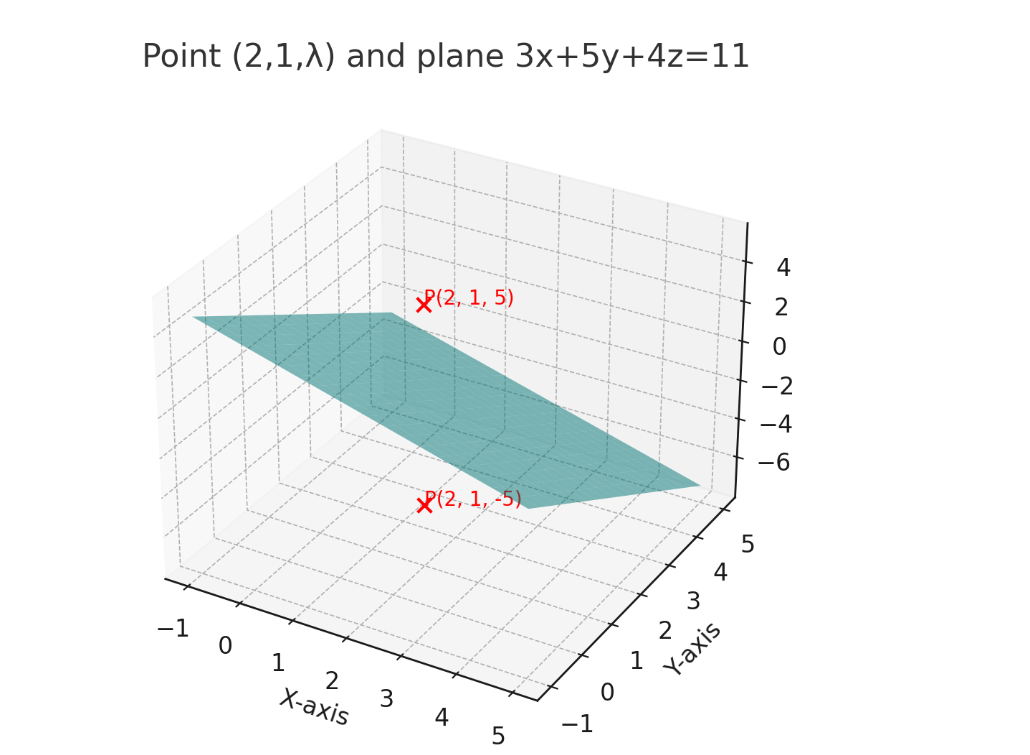
\includegraphics[width=0.90\linewidth]{figs/image.png}
    \caption{Image}
    \label{fig:placeholder}
\end{figure}
\end{frame}

\begin{frame}[fragile]{C code}
\begin{lstlisting}[language = c]
#include <stdio.h>
#include <math.h>
#include <stdlib.h>  // For fabs()

int main() {
    // Plane: 3x + 5y + 4z = 11
    double n[] = {3, 5, 4};  // Normal vector components
    double d_plane = 11;     // Plane constant
    double distance = 2 * sqrt(2); // Given distance

    // Point: (2, 1, lambda)
    double x = 2, y = 1;
    double lambda;

    // Distance formula: d = |n . p - d_plane| / ||n||
    // ||n|| = sqrt(3^2 + 5^2 + 4^2) = sqrt(50) = 5*sqrt(2)
    double norm_n = sqrt(n[0]*n[0] + n[1]*n[1] + n[2]*n[2]); 
\end{lstlisting}
\end{frame}

\begin{frame}[fragile]{C code}
\begin{lstlisting}[language = c]
    // Solve for lambda: |n . p - d_plane| / ||n|| = distance
    // n . p = 3*2 + 5*1 + 4*lambda = 11 + 4*lambda
    // |11 + 4*lambda - 11| / (5*sqrt(2)) = 2*sqrt(2)
    // => |4*lambda| / (5*sqrt(2)) = 2*sqrt(2)
    // => |lambda| = 5
    lambda = 5;
    printf("Lambda = %.2f or %.2f\n", lambda, -lambda);

    return 0;
}
\end{lstlisting}
\end{frame}

\begin{frame}[fragile]{Python code}
\begin{lstlisting}
import math

# Plane: 3x + 5y + 4z = 11
n = [3, 5, 4]  # Normal vector
d_plane = 11   # Plane constant
distance = 2 * math.sqrt(2)  # Given distance

# Point: (2, 1, lambda)
x, y = 2, 1

# Norm of the normal vector
norm_n = math.sqrt(n[0]**2 + n[1]**2 + n[2]**2)  # ||n||

lambda_val = 5
print(f"Lambda = {lambda_val} or {-lambda_val}")

\end{lstlisting}
\end{frame}
\end{document}